\section{Formal review}
To ensure the quality of the code and the correctness of the tests, we made use of formal reviews.
A formal review is a process that belongs to the static white-box testing category.
A formal review contains four essential elements \cite{SoftwareTesting}:
\begin{itemize}\label{formalreview}
    \item Identify problems
    \item Follow rules
    \item Prepare
    \item Write a report
\end{itemize}
The goal of the review is to find problems or deficiencies in the software, with criticism directed at the design or the code itself.
Rules should be established regarding the process, such that they can be followed during a formal review.
An example of a rule could be defining the maximum amount of code to be reviewed at one time, or how many reviewers should examine the code.
Each participant in the review should be prepared for it, such that they can contribute.
Depending on the type of review, the participants could have different roles, and this should be known before the review begins, such that the roles can be actively fulfilled.
The review group should ultimately produce a report summarizing the results of the review, such that other developers can become aware of the results. 

\subsection{Our formal review process}
Initially when reviewing our code we would have two reviewers individually review the code and write comments and suggested changes. 
This would be done by creating a pull request (PR) to the develop branch and the author would then assign two reviewers.
When a review had been submitted by the reviewer, the author would go through the list of suggested changes to the code and fix the code or ask clarifying questions to the reviewer.
After two reviewers had accepted the PR it could be merged to the develop branch by the author. 
\\\\
To further ensure that the quality of the code that is pushed to develop is of acceptable quality we use continuous integration (CI).
The CI ensures that the project is able to build without any errors, and that the unit tests succeed. 
That way we can be sure that the develop branch is never a broken build, since it will try to run both the original branch, and the develop branch with the new changes merged in.
Additionally, we use a linter that is configured to test that the code follows our internally defined rules and coding standards. 
In addition to this, the CI runs the linter, and if the code does not follow the standards set it will report an error.
\begin{figure}[H]
    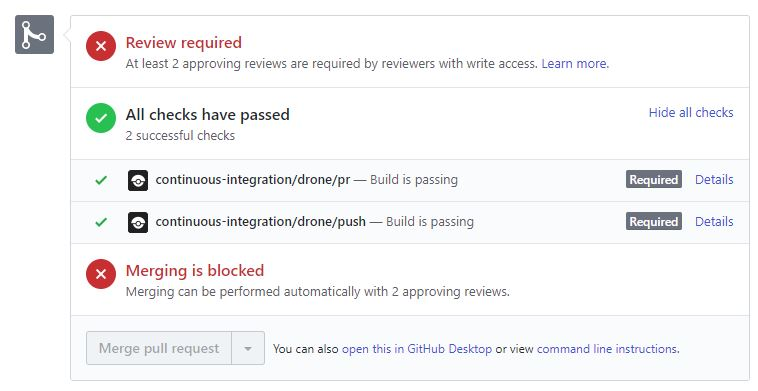
\includegraphics[width=\linewidth]{/ci.JPG}
    \caption{The CI has to succeed for a PR to be merged}
    \label{fig:continous-integration}
\end{figure}
\noindent
During the later stages of the project we decided to change our approach to formal reviews.
Rather than have two developers individually review a PR, we strove to have the developers get together for the review.
This would ensure more discussions arose based on the PR, and increase the overall quality of the review, since it would encourage the developers to do a deeper reflection on the code.
\\\\
In terms of the four essential elements defined in \autoref{formalreview}, our process achieves these elements.
We did not directly write a report, as this element is mostly necessary for larger systems developed by larger teams.
Instead, the results of our reviews were made available through comments and suggestions to the PRs, such that other developers could access them.
\begin{figure}[H]
    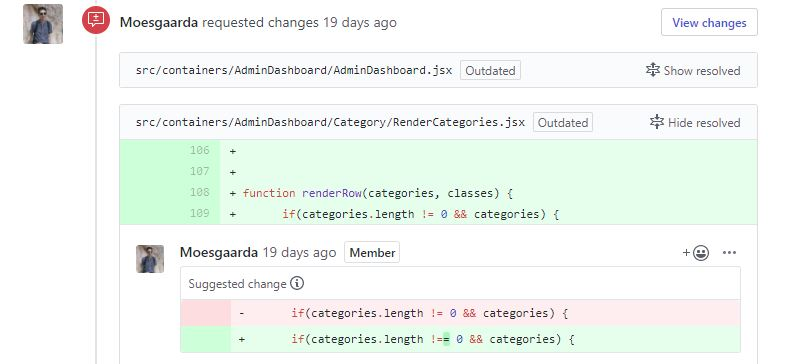
\includegraphics[width=\linewidth]{/commentonpr.JPG}
    \caption{An example of a comment on a PR}
    \label{fig:comment-on-pr}
\end{figure}
